% ==============================================================================
% Kapitola 2: Karnaughova mapa - hra na hledání rozdílů
% ==============================================================================
\section{Karnaughova mapa (hledání rozdílů)}

\begin{hack}[K-Mapa je jen hra na hledání rozdílů]
\textbf{Tři kroky:}
\begin{enumerate}
\item \textbf{Vyplň mapu:} podle mintermů vyznač 1
\item \textbf{Seskup 1:} zakroužkuj je (čím větší skupina, tím lépe)
\item \textbf{Napiš člen:} zapiš proměnné, které se ve skupině nemění
\end{enumerate}
\end{hack}

\subsection{Šablona pro 4 proměnné (okopíruj)}

\begin{center}
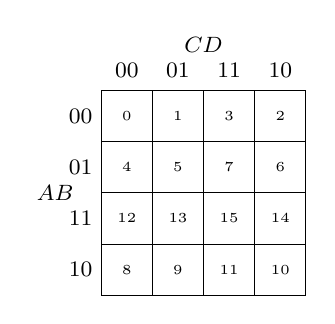
\begin{tikzpicture}[scale=0.65]
\draw (0,0) grid (4,4);
% Popisky sloupců CD
\node at (0.5, 4.4) {\footnotesize 00};
\node at (1.5, 4.4) {\footnotesize 01};
\node at (2.5, 4.4) {\footnotesize 11};
\node at (3.5, 4.4) {\footnotesize 10};
\node at (2, 4.9) {\footnotesize $CD$};
% Popisky řádků AB
\node at (-0.4, 3.5) {\footnotesize 00};
\node at (-0.4, 2.5) {\footnotesize 01};
\node at (-0.4, 1.5) {\footnotesize 11};
\node at (-0.4, 0.5) {\footnotesize 10};
\node at (-0.9, 2) {\footnotesize $AB$};
% Indexy
\node at (0.5,3.5) {\tiny 0};
\node at (1.5,3.5) {\tiny 1};
\node at (2.5,3.5) {\tiny 3};
\node at (3.5,3.5) {\tiny 2};
\node at (0.5,2.5) {\tiny 4};
\node at (1.5,2.5) {\tiny 5};
\node at (2.5,2.5) {\tiny 7};
\node at (3.5,2.5) {\tiny 6};
\node at (0.5,1.5) {\tiny 12};
\node at (1.5,1.5) {\tiny 13};
\node at (2.5,1.5) {\tiny 15};
\node at (3.5,1.5) {\tiny 14};
\node at (0.5,0.5) {\tiny 8};
\node at (1.5,0.5) {\tiny 9};
\node at (2.5,0.5) {\tiny 11};
\node at (3.5,0.5) {\tiny 10};
\end{tikzpicture}
\end{center}

\textbf{Pořadí Grayova kódu: 00, 01, 11, 10} (nauč se)

\subsection{Jak vyplňovat mapu}

\begin{hack}[Kam patří která proměnná?]
\textbf{Oblasti pro ABCD ve 4-proměnné mapě:}
\begin{itemize}
\item $A=1$: spodní dva řádky (řádky 11, 10)
\item $B=1$: prostřední dva řádky (řádky 01, 11)
\item $C=1$: prostřední dva sloupce (sloupce 01, 11)
\item $D=1$: pravé dva sloupce (sloupce 11, 10)
\end{itemize}

\textbf{Negace:} $\bar{A}$ znamená oblast $A=0$.
\end{hack}

\subsection{Seskupování bez přemýšlení}

\begin{hack}[Čtyři povinné vzory seskupování]
\textbf{1. Čtyři rohy} = $\bar{B}\bar{D}$
\begin{center}
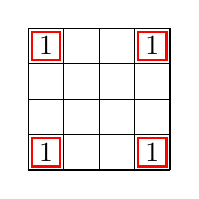
\begin{tikzpicture}[scale=0.45]
\draw (0,0) grid (4,4);
\node at (0.5,3.5) {1}; \node at (3.5,3.5) {1};
\node at (0.5,0.5) {1}; \node at (3.5,0.5) {1};
\draw[red,thick] (0.1,3.1) rectangle (0.9,3.9);
\draw[red,thick] (3.1,3.1) rectangle (3.9,3.9);
\draw[red,thick] (0.1,0.1) rectangle (0.9,0.9);
\draw[red,thick] (3.1,0.1) rectangle (3.9,0.9);
\end{tikzpicture}
\end{center}

\textbf{2. Celý řádek} = mění se jen AB
\begin{center}
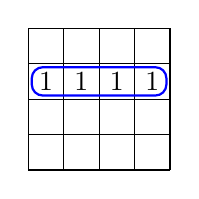
\begin{tikzpicture}[scale=0.45]
\draw (0,0) grid (4,4);
\node at (0.5,2.5) {1}; \node at (1.5,2.5) {1};
\node at (2.5,2.5) {1}; \node at (3.5,2.5) {1};
\draw[blue,thick,rounded corners] (0.1,2.1) rectangle (3.9,2.9);
\end{tikzpicture}
\end{center}

\textbf{3. Blok 2x2 (4 buňky)} = odstraní dvě proměnné

\textbf{4. Přes okraj (nahoru/dolů nebo vlevo/vpravo)} = skupiny mohou přecházet hranice
\end{hack}

\subsection{Pravidla seskupování}

\begin{pitfall}[Tři železná pravidla]
\begin{enumerate}
\item Velikost skupiny musí být \textbf{mocnina dvou}: 1, 2, 4, 8, 16
\item \textbf{Čím větší, tím lepší} (odstraní více proměnných)
\item Každá 1 musí být \textbf{pokryta alespoň jednou}
\end{enumerate}
\end{pitfall}

\subsection{Jak psát výraz ze skupiny}

\begin{hack}[Zapiš to, co se ve skupině nemění]
\textbf{Sleduj hodnoty proměnných ve skupině:}
\begin{itemize}
\item vždy 1 $\to$ napiš proměnnou
\item vždy 0 $\to$ napiš negovanou proměnnou
\item někdy 0 někdy 1 $\to$ vynech (zruší se)
\end{itemize}

\textbf{Příklad:} skupina v AB=01, CD=libovolně
\begin{itemize}
\item A je vždy 0 $\to$ napiš $\bar{A}$
\item B je vždy 1 $\to$ napiš $B$
\item C a D se mění $\to$ vynech
\item \textbf{Výsledek: $\bar{A}B$}
\end{itemize}
\end{hack}

\subsection{Tajemství XOR}

\begin{hack}[Šachovnice = XOR]
Pokud se v K-map střídají 1 a 0 jako na šachovnici:

\begin{center}
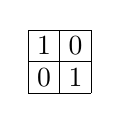
\begin{tikzpicture}[scale=0.4]
\draw (0,0) grid (2,2);
\node at (0.5,1.5) {1}; \node at (1.5,1.5) {0};
\node at (0.5,0.5) {0}; \node at (1.5,0.5) {1};
\end{tikzpicture}
\end{center}

\textbf{Napiš rovnou:} $A \oplus B$ (XOR)

Tady to \textbf{nejde dál zjednodušit}; neztrácej čas seskupováním.
\end{hack}

\subsection{Don't care}

\begin{keybox}[X můžeš brát jako 1 nebo 0]
\begin{itemize}
\item Pokud zvětší skupinu $\to$ ber jako 1
\item Jinak $\to$ ber jako 0 a ignoruj
\end{itemize}
Cíl: udělat skupiny co největší.
\end{keybox}
